\documentclass[11pt,a4paper]{article}
\usepackage[top=2cm, bottom=2.3cm, left=1.8cm, right=1.8cm, headsep=0.8cm]{geometry}
\usepackage{amsmath,amssymb,amsfonts}
\usepackage{graphicx}
\graphicspath{{images/}{public/exam-images/SohanMock/}{./}}
\usepackage{enumitem}
\usepackage{fancyhdr}
\usepackage[table]{xcolor}
\usepackage{tcolorbox}
\tcbuselibrary{breakable,skins}
\usepackage{tabularx}
\usepackage{multicol}

% High-Contrast Modern Color Palette
\definecolor{primaryDark}{RGB}{12, 32, 84}       % Midnight Navy
\definecolor{primaryBlue}{RGB}{18, 72, 160}      % Solid Royal Blue
\definecolor{goldAccent}{RGB}{255, 215, 0}       % Gold highlight
\definecolor{l1Green}{RGB}{14, 120, 62}          % Vivid Forest Green
\definecolor{l2Amber}{RGB}{205, 80, 0}           % Rich Amber
\definecolor{l3Crimson}{RGB}{180, 20, 20}        % Deep Crimson Red
\definecolor{cardBg}{RGB}{250, 252, 255}         % Crisp Card Background
\definecolor{cardBorder}{RGB}{130, 170, 220}     % Steel Blue Border
\definecolor{tableStripe}{RGB}{242, 246, 252}    % Alternating Table Row
\definecolor{tableDarkHeader}{RGB}{12, 32, 84}   % Dark Table Header

% Page styling
\pagestyle{fancy}
\fancyhf{}
\setlength{\headheight}{16pt}
\fancyhead[L]{\small\textsf{\textbf{\textcolor{primaryDark}{Sohan Mocks Series}} $\vert$ \textbf{\textcolor{primaryBlue}{Physics: Work, Power \& Energy}}}}
\fancyhead[R]{\small\textsf{\textbf{\textcolor{l1Green}{Max Marks: 100 $\vert$ 60 Mins}}}}
\fancyfoot[C]{\textbf{\textsf{\thepage}}}
\renewcommand{\headrulewidth}{0.8pt}
\renewcommand{\footrulewidth}{0.4pt}

% Custom tcolorbox styles
\tcbset{
  dayheader/.style={
    colback=primaryDark,
    coltext=white,
    boxrule=0pt,
    arc=3mm,
    left=14pt, right=14pt, top=10pt, bottom=10pt
  },
  sectionbanner/.style={
    colback=primaryBlue,
    coltext=white,
    boxrule=0pt,
    arc=2mm,
    left=10pt, right=10pt, top=6pt, bottom=6pt
  },
  solbox/.style={
    enhanced,
    breakable,
    colback=cardBg,
    colframe=cardBorder,
    boxrule=1.0pt,
    arc=2mm,
    left=10pt, right=10pt, top=7pt, bottom=7pt
  }
}

\begin{document}

% ==================== TEST HEADER BANNER ====================
\begin{tcolorbox}[dayheader]
\begin{center}
  {\Large \textbf{\textsf{\textcolor{goldAccent}{SOHAN MOCKS TEST SERIES}}}}\\[3pt]
  {\LARGE \textbf{\textsf{TOPICAL SPECIAL: WORK, POWER \& ENERGY (JEE FULL MOCK)}}}\\[5pt]
  {\normalsize \textbf{\textsf{Core Domains:}} Variable Force Integrals $\vert$ Vertical Circular Motion $\vert$ Conservative Fields $\vert$ Springs $\vert$ Collisions}\\[3pt]
  {\footnotesize \textbf{Exam Pattern:} 25 Questions (20 MCQs $+4/-1$ + 5 Numerical $+4/0$) \quad $\vert$ \quad \textbf{Time:} 60 Minutes \quad $\vert$ \quad \textbf{Max Marks:} 100}
\end{center}
\end{tcolorbox}

\vspace{6pt}

% ==================== SECTION I: SINGLE CORRECT CHOICE ====================
\begin{tcolorbox}[sectionbanner]
  {\large \textbf{\textsf{SECTION I: SINGLE CORRECT CHOICE TYPE (Q01 -- Q20)}}} \hfill {\small \textbf{Marking: $+4$ / $-1$}}
\end{tcolorbox}
\vspace{4pt}

\begin{enumerate}[label=\textbf{\arabic*.},leftmargin=18pt,itemsep=12pt]

  \item A force $\vec{F} = (3x^2\hat{i} + 4y\hat{j})\text{ N}$ acts on a particle of mass $2\text{ kg}$, causing it to move from the origin $(0,0)\text{ m}$ to the point $(2,3)\text{ m}$ in the $xy$-plane. The work done by this force on the particle is:
  \begin{multicols}{4}
    \begin{enumerate}[label=(\Alph*)]
      \item $18\text{ J}$
      \item $26\text{ J}$
      \item $24\text{ J}$
      \item $32\text{ J}$
    \end{enumerate}
  \end{multicols}

  \item The potential energy of a two-particle interaction as a function of their separation $x$ is given by $U(x) = \dfrac{a}{x^{12}} - \dfrac{b}{x^6}$, where $a$ and $b$ are positive constants, as shown in the potential energy curve. The equilibrium separation $x_0$ and the depth of the potential well $U_{\min}$ (minimum potential energy) are:
  \begin{center}
    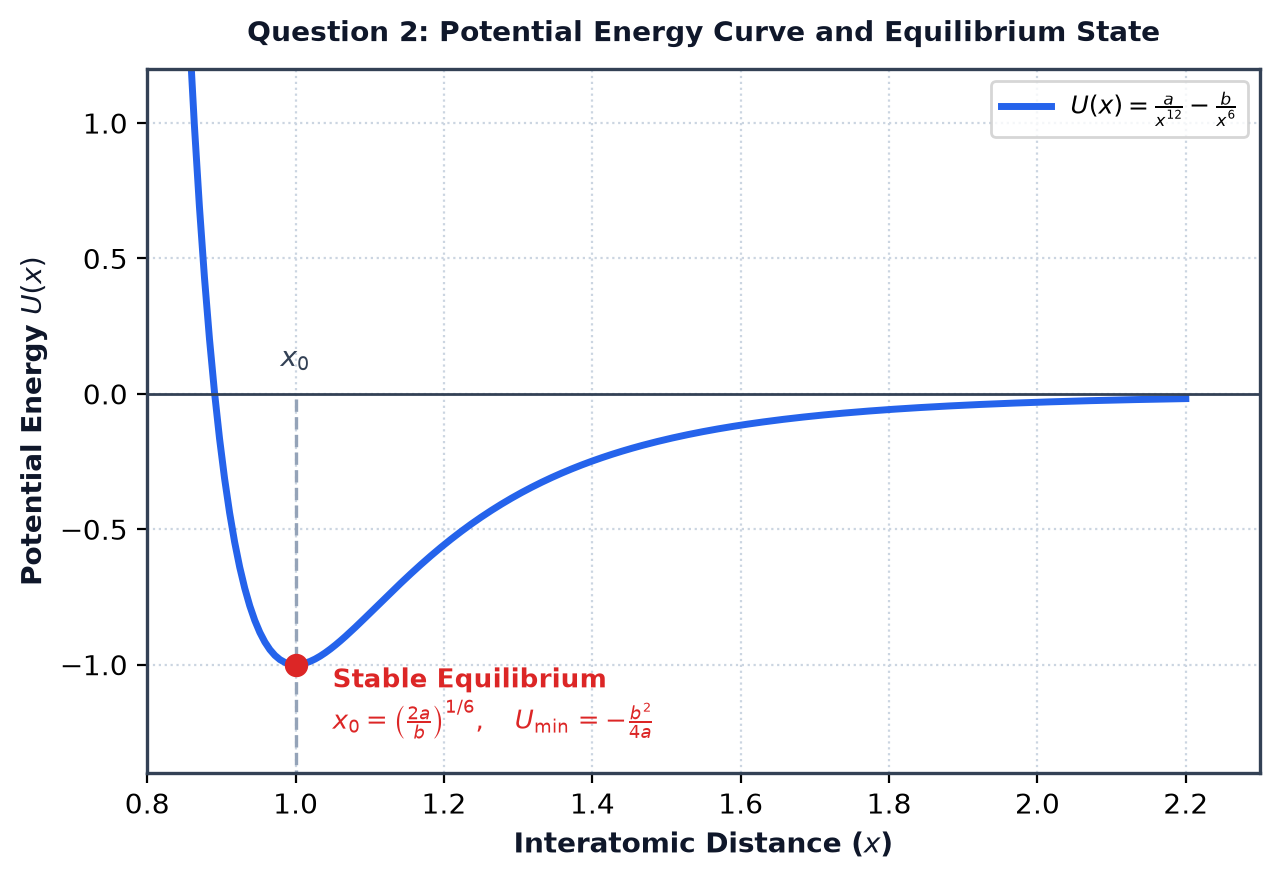
\includegraphics[width=0.38\textwidth]{images/sohan_wpe_q02_potential_curve.png}
  \end{center}
  \begin{enumerate}[label=(\Alph*)]
    \item $x_0 = \left(\dfrac{a}{b}\right)^{1/6}, \quad U_{\min} = -\dfrac{b^2}{2a}$
    \item $x_0 = \left(\dfrac{2a}{b}\right)^{1/6}, \quad U_{\min} = -\dfrac{b^2}{2a}$
    \item $x_0 = \left(\dfrac{2a}{b}\right)^{1/6}, \quad U_{\min} = -\dfrac{b^2}{4a}$
    \item $x_0 = \left(\dfrac{a}{2b}\right)^{1/6}, \quad U_{\min} = -\dfrac{b^2}{4a}$
  \end{enumerate}

  \item A small bob of mass $m$ attached to a light inextensible string of length $L$ is whirled in a vertical circle. The bob is imparted the minimum critical speed $v_0 = \sqrt{5gL}$ at the lowest point $A$ required to complete the full vertical circle, as shown in the diagram. The ratio of the tension in the string at the lowest point $A$ to the tension when the string becomes horizontal at point $B$ ($\dfrac{T_A}{T_B}$) is:
  \begin{center}
    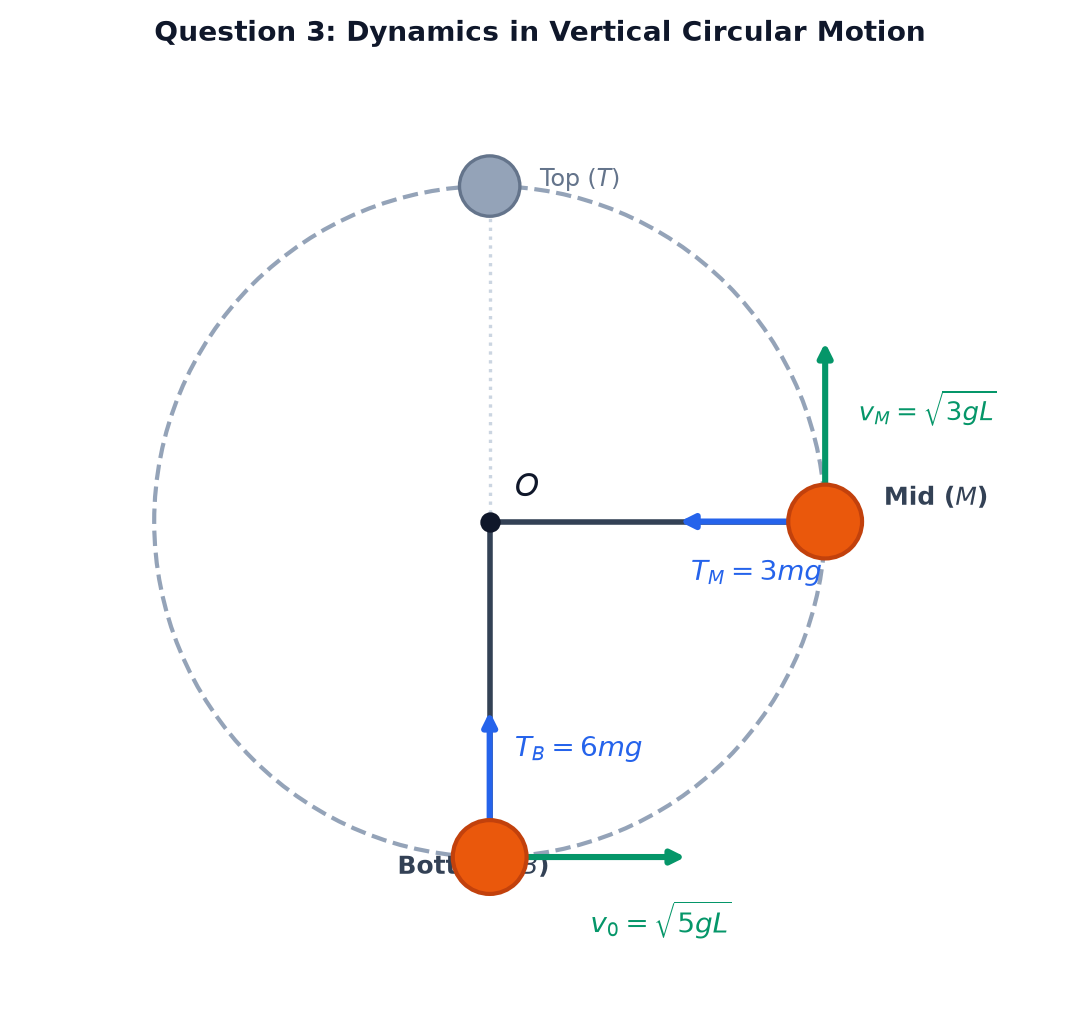
\includegraphics[width=0.32\textwidth]{images/sohan_wpe_q03_vertical_circle.png}
  \end{center}
  \begin{multicols}{4}
    \begin{enumerate}[label=(\Alph*)]
      \item $2$
      \item $3$
      \item $\dfrac{5}{3}$
      \item $\dfrac{7}{3}$
    \end{enumerate}
  \end{multicols}

  \item A block of mass $m = 2\text{ kg}$ is released from rest at the top of a rough inclined plane of length $L = 5\text{ m}$ and angle of inclination $\theta = 37^\circ$ ($\sin 37^\circ \approx 0.6, \cos 37^\circ \approx 0.8$). The coefficient of kinetic friction between the block and the incline is $\mu = 0.25$. Taking $g = 10\text{ m/s}^2$, the speed of the block when it reaches the bottom of the incline is:
  \begin{center}
    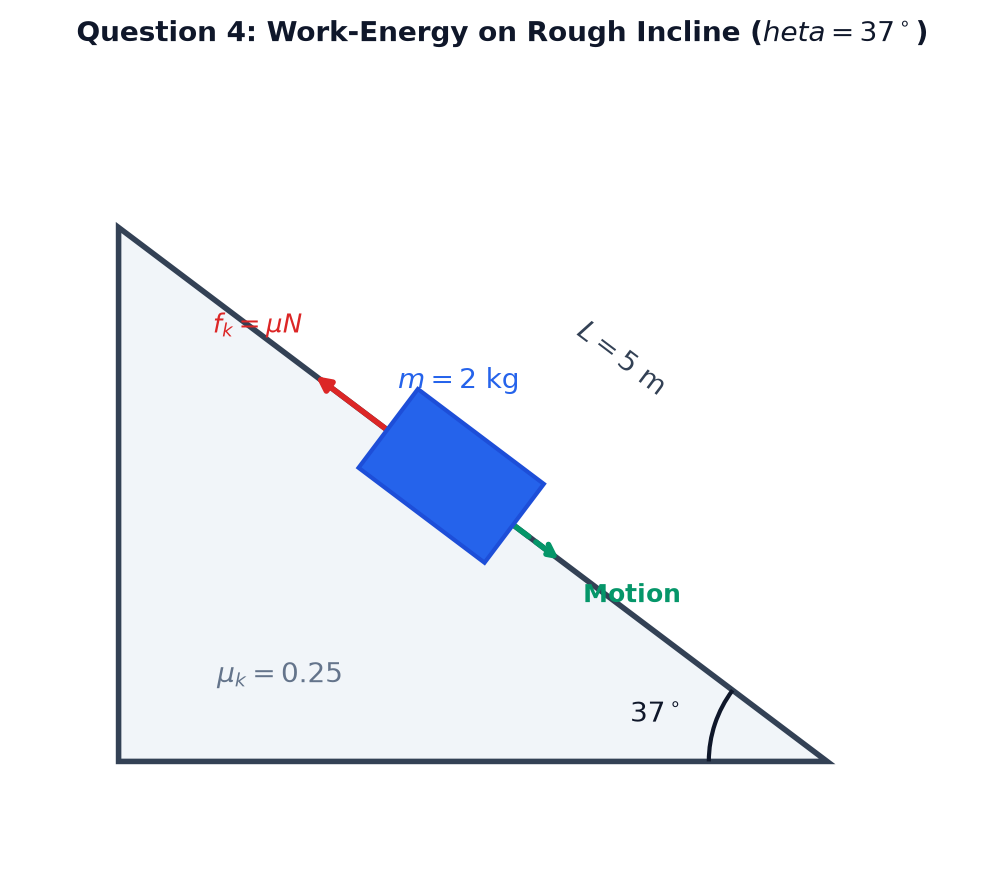
\includegraphics[width=0.40\textwidth]{images/sohan_wpe_q04_incline_friction.png}
  \end{center}
  \begin{multicols}{2}
    \begin{enumerate}[label=(\Alph*)]
      \item $6\text{ m/s}$
      \item $4\sqrt{5}\text{ m/s}$
      \item $8\text{ m/s}$
      \item $2\sqrt{10}\text{ m/s}$
    \end{enumerate}
  \end{multicols}

  \item A vehicle of mass $m$ starts from rest and is driven along a straight horizontal road by an engine delivering constant mechanical power $P$. Assuming no resistive losses, the displacement $x$ of the vehicle from the start as a function of time $t$ is proportional to:
  \begin{multicols}{4}
    \begin{enumerate}[label=(\Alph*)]
      \item $t^{1/2}$
      \item $t^{3/2}$
      \item $t^2$
      \item $t^{5/2}$
    \end{enumerate}
  \end{multicols}

  \item A block of mass $m$ moving with speed $v$ on a rough horizontal surface hits an uncompressed ideal spring of force constant $k$ fixed to a rigid vertical wall, as depicted in the figure. A constant frictional force $f$ opposes the motion of the block throughout. The maximum compression $x$ of the spring is:
  \begin{center}
    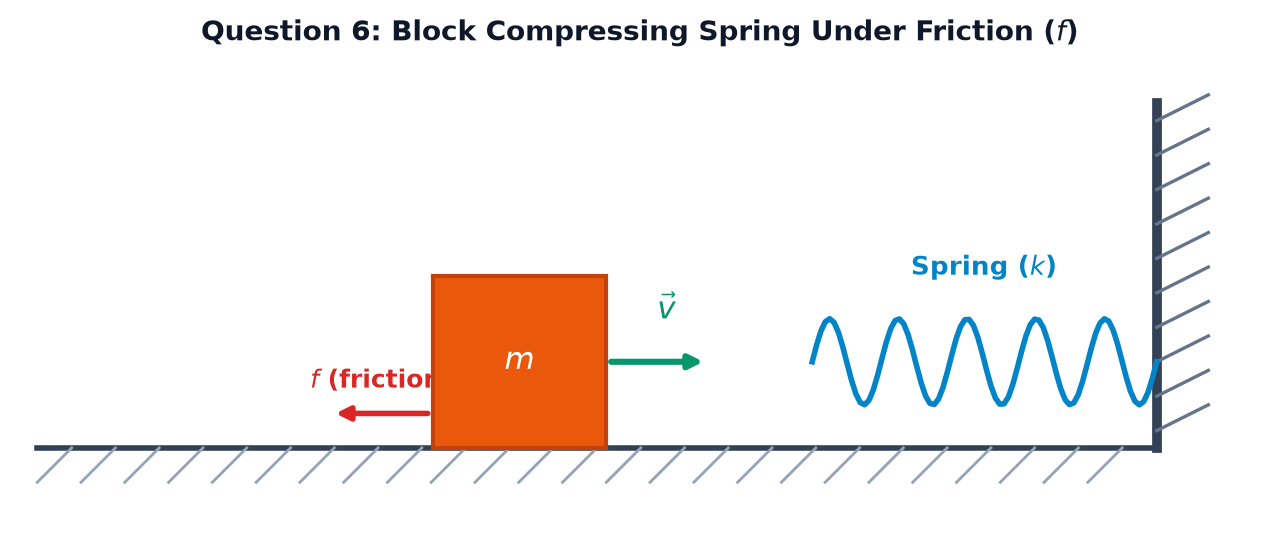
\includegraphics[width=0.38\textwidth]{images/sohan_wpe_q06_spring_block.png}
  \end{center}
  \begin{enumerate}[label=(\Alph*)]
    \item $\dfrac{\sqrt{f^2 + km v^2} - f}{k}$
    \item $\dfrac{\sqrt{f^2 + 2km v^2} - f}{k}$
    \item $\dfrac{\sqrt{f^2 + km v^2} + f}{k}$
    \item $\sqrt{\dfrac{m v^2 - 2fx}{k}}$
  \end{enumerate}

  \item The potential energy of a particle in a conservative force field is given by $U(x, y) = 3x^2 y - 7x + 2y^3$, where $x$ and $y$ are in meters and $U$ is in Joules. The conservative force $\vec{F}$ acting on the particle at the coordinates $(1\text{ m}, -1\text{ m})$ is:
  \begin{multicols}{2}
    \begin{enumerate}[label=(\Alph*)]
      \item $(-13\hat{i} + 9\hat{j})\text{ N}$
      \item $(13\hat{i} + 9\hat{j})\text{ N}$
      \item $(13\hat{i} - 9\hat{j})\text{ N}$
      \item $(7\hat{i} - 3\hat{j})\text{ N}$
    \end{enumerate}
  \end{multicols}

  \item A small block of mass $m$ slides down from rest along a frictionless track from a height $h$ and enters a vertical circular loop of radius $R$, as shown in the diagram. If the normal reaction force exerted by the track on the block at the highest point of the loop is exactly equal to the block's weight ($N_{\text{top}} = mg$), the release height $h$ must be:
  \begin{center}
    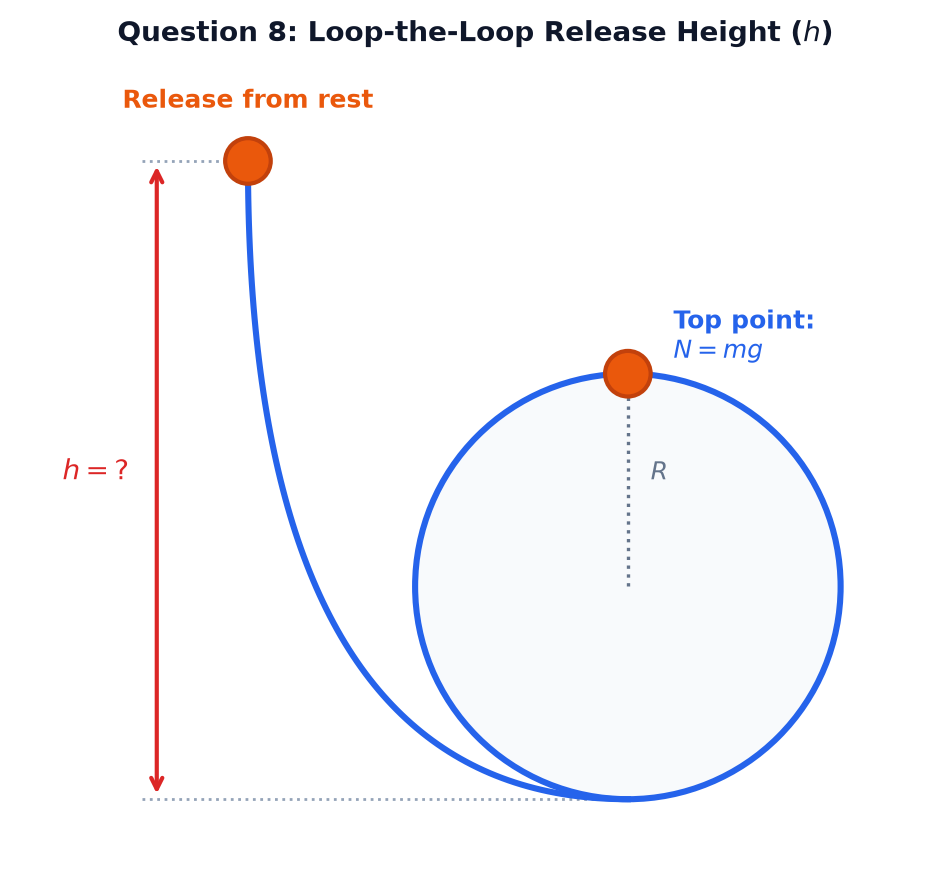
\includegraphics[width=0.36\textwidth]{images/sohan_wpe_q08_loop_the_loop.png}
  \end{center}
  \begin{multicols}{4}
    \begin{enumerate}[label=(\Alph*)]
      \item $2.5R$
      \item $3R$
      \item $3.5R$
      \item $4R$
    \end{enumerate}
  \end{multicols}

  \item An electric crane lifts a cargo container of mass $M = 500\text{ kg}$ vertically upwards from rest with a uniform acceleration of $a = 2\text{ m/s}^2$. Taking $g = 10\text{ m/s}^2$, the instantaneous power delivered by the crane cable at $t = 5\text{ s}$ after starting the lift is:
  \begin{multicols}{4}
    \begin{enumerate}[label=(\Alph*)]
      \item $60\text{ kW}$
      \item $50\text{ kW}$
      \item $10\text{ kW}$
      \item $75\text{ kW}$
    \end{enumerate}
  \end{multicols}

  \item A motor pump is used to continuously pump water through a pipe of cross-sectional area $A$. If the pump is required to discharge water at $n$ times the original mass flow rate through the same nozzle, the power delivered by the motor must be increased by a factor of:
  \begin{multicols}{4}
    \begin{enumerate}[label=(\Alph*)]
      \item $n$
      \item $n^2$
      \item $n^{3/2}$
      \item $n^3$
    \end{enumerate}
  \end{multicols}

  \item Two blocks of masses $m_1$ and $m_2$ connected by a light spring of force constant $k$ lie on a smooth horizontal surface, initially at rest with the spring in its natural state, as illustrated. A constant horizontal force $F$ is applied to mass $m_1$ directing away from $m_2$. The maximum elongation produced in the spring is:
  \begin{center}
    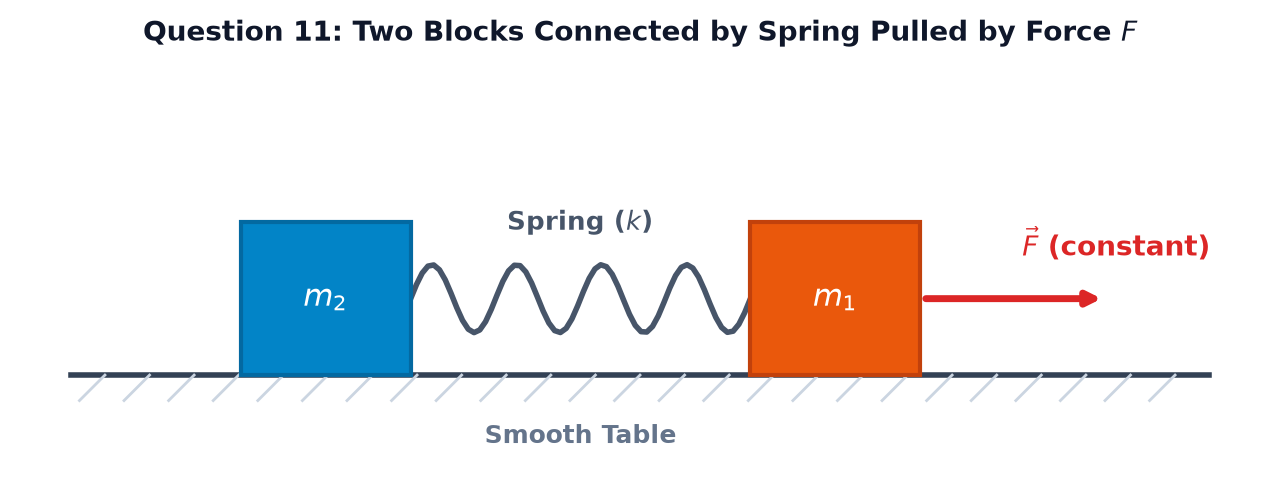
\includegraphics[width=0.38\textwidth]{images/sohan_wpe_q11_two_blocks_spring.png}
  \end{center}
  \begin{multicols}{2}
    \begin{enumerate}[label=(\Alph*)]
      \item $\dfrac{F m_2}{k(m_1 + m_2)}$
      \item $\dfrac{2F m_2}{k(m_1 + m_2)}$
      \item $\dfrac{2F}{k}$
      \item $\dfrac{2F m_1}{k(m_1 + m_2)}$
    \end{enumerate}
  \end{multicols}

  \item A uniform flexible chain of length $L$ and total mass $M$ is placed on a smooth horizontal table such that a fraction $\dfrac{1}{3}$ of its length hangs vertically over the edge of the table, as shown in the diagram. The minimum work done by an external agent to slowly pull the hanging part back onto the table is:
  \begin{center}
    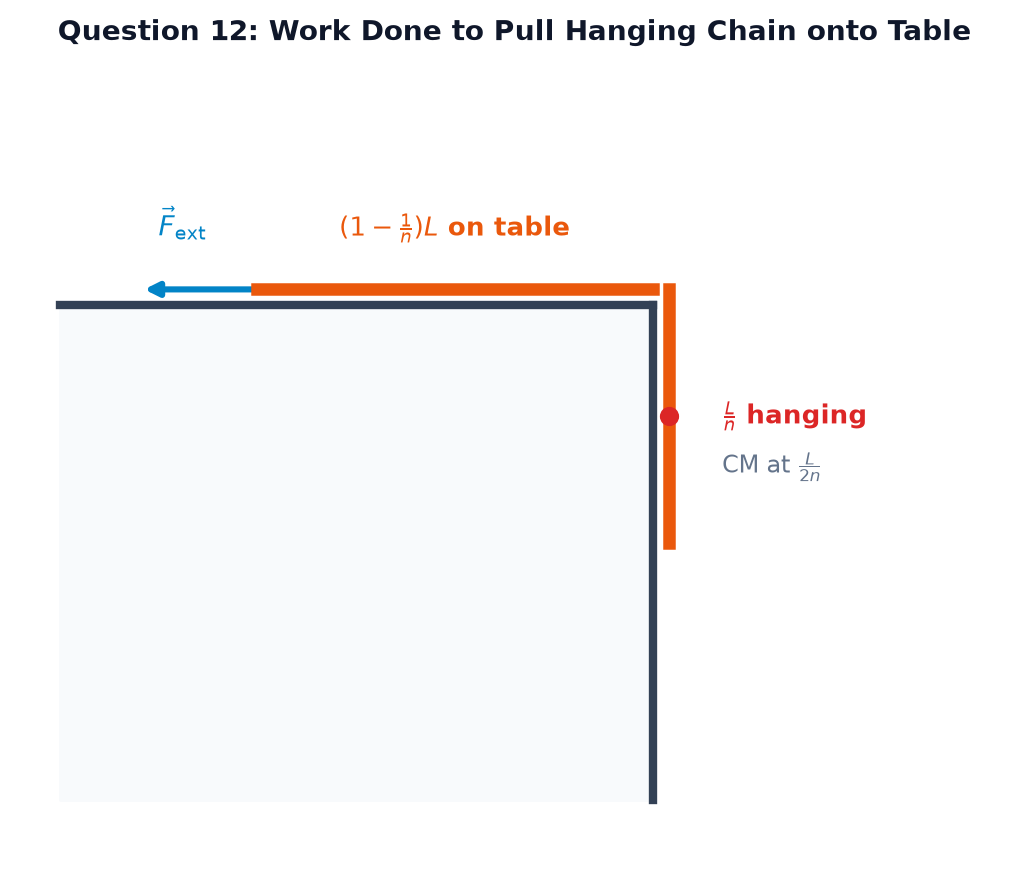
\includegraphics[width=0.36\textwidth]{images/sohan_wpe_q12_hanging_chain.png}
  \end{center}
  \begin{multicols}{2}
    \begin{enumerate}[label=(\Alph*)]
      \item $\dfrac{MgL}{9}$
      \item $\dfrac{MgL}{6}$
      \item $\dfrac{MgL}{18}$
      \item $\dfrac{MgL}{36}$
    \end{enumerate}
  \end{multicols}

  \item A force field is given by $\vec{F} = (y\hat{i} + x^2\hat{j})\text{ N}$. A particle is moved from the origin $(0,0)$ to the point $(1,1)\text{ m}$ along two straight line segments: first along the $x$-axis from $(0,0)$ to $(1,0)$, and then parallel to the $y$-axis from $(1,0)$ to $(1,1)$. The work done by this force along this path is:
  \begin{multicols}{2}
    \begin{enumerate}[label=(\Alph*)]
      \item $1\text{ J}$
      \item $\dfrac{5}{6}\text{ J}$
      \item $\dfrac{1}{2}\text{ J}$
      \item $2\text{ J}$
    \end{enumerate}
  \end{multicols}

  \item A simple pendulum bob of mass $m$ attached to a light rigid string of length $L$ is released from rest from the horizontal position ($\theta_0 = 90^\circ$ from vertical). The tension in the string when the bob reaches a position making an angle of $60^\circ$ with the downward vertical is:
  \begin{multicols}{2}
    \begin{enumerate}[label=(\Alph*)]
      \item $2mg$
      \item $\dfrac{5}{2}mg$
      \item $\dfrac{1}{2}mg$
      \item $\dfrac{3}{2}mg$
    \end{enumerate}
  \end{multicols}

  \item An ideal spring has a natural length $L_0$. The work done in stretching the spring from an elongation of $10\text{ cm}$ to $20\text{ cm}$ is $W_1$, and the work done in stretching it further from an elongation of $20\text{ cm}$ to $30\text{ cm}$ is $W_2$. The ratio $\dfrac{W_1}{W_2}$ is:
  \begin{multicols}{4}
    \begin{enumerate}[label=(\Alph*)]
      \item $\dfrac{1}{2}$
      \item $\dfrac{2}{3}$
      \item $\dfrac{3}{5}$
      \item $\dfrac{1}{3}$
    \end{enumerate}
  \end{multicols}

  \item A particle of mass $m = 1\text{ kg}$ moves along the $x$-axis in a potential field $U(x) = 2x^4 - 4x^2 + 5$, where $x$ is in meters and $U$ is in Joules. For small amplitude oscillations about one of its positions of stable equilibrium, the angular frequency of oscillation $\omega$ is:
  \begin{multicols}{2}
    \begin{enumerate}[label=(\Alph*)]
      \item $4\text{ rad/s}$
      \item $2\text{ rad/s}$
      \item $2\sqrt{2}\text{ rad/s}$
      \item $8\text{ rad/s}$
    \end{enumerate}
  \end{multicols}

  \item A car of mass $m$ travels along a horizontal circular track of radius $R$ starting from rest at $t = 0$. Its tangential acceleration $a_t$ is constant throughout. The instantaneous power $P(t)$ delivered by the net resultant force to the car as a function of time $t$ is:
  \begin{enumerate}[label=(\Alph*)]
    \item $\dfrac{1}{2} m a_t^2 t$
    \item $m a_t^2 t$
    \item $m a_t^2 t \sqrt{1 + \left(\dfrac{a_t t^2}{R}\right)^2}$
    \item $\dfrac{m a_t^3 t^2}{R}$
  \end{enumerate}

  \item A small rubber ball is dropped from an initial height $h_0 = 10\text{ m}$ onto a fixed horizontal hard floor. The coefficient of restitution for each impact with the floor is $e = 0.5$. The total distance traveled by the ball until it ceases to bounce is:
  \begin{multicols}{2}
    \begin{enumerate}[label=(\Alph*)]
      \item $20\text{ m}$
      \item $15\text{ m}$
      \item $\dfrac{40}{3}\text{ m}$
      \item $\dfrac{50}{3}\text{ m}$
    \end{enumerate}
  \end{multicols}

  \item A block sliding on a rough horizontal surface with an initial velocity $v$ comes to rest after covering a distance $s_1$ due to uniform kinetic friction. If the initial velocity of the block is increased to $3v$ under identical surface conditions, the stopping distance becomes:
  \begin{multicols}{4}
    \begin{enumerate}[label=(\Alph*)]
      \item $3 s_1$
      \item $6 s_1$
      \item $9 s_1$
      \item $27 s_1$
    \end{enumerate}
  \end{multicols}

  \item Two springs $A$ and $B$ have spring constants $k_A$ and $k_B$ respectively, such that $k_A = 2 k_B$. Both springs are initially unstretched. If both springs are stretched by applying equal pulling forces $F$, the ratio of the work done on spring $A$ to the work done on spring $B$ ($\dfrac{W_A}{W_B}$) is:
  \begin{multicols}{4}
    \begin{enumerate}[label=(\Alph*)]
      \item $\dfrac{1}{2}$
      \item $2$
      \item $4$
      \item $\dfrac{1}{4}$
    \end{enumerate}
  \end{multicols}

\end{enumerate}

\vspace{10pt}

% ==================== SECTION II: NUMERICAL VALUE TYPE ====================
\begin{tcolorbox}[sectionbanner]
  {\large \textbf{\textsf{SECTION II: NUMERICAL VALUE TYPE (Q21 -- Q25)}}} \hfill {\small \textbf{Marking: $+4$ / $0$ (No Negative)}}
\end{tcolorbox}
\vspace{4pt}

\begin{enumerate}[label=\textbf{\arabic*.},leftmargin=18pt,itemsep=12pt,resume]

  \item A small particle attached to a light inextensible string of length $L$ is projected horizontally from the lowest point with speed $v_0 = \sqrt{3gL}$. The particle moves in a vertical plane until the string becomes slack at a height $h = \dfrac{N}{3}L$ above the lowest point. Find the integer value of $N$.

  \item A block of mass $m = 2\text{ kg}$ is released from rest from a height $h = 40\text{ cm}$ above the top of an uncompressed vertical spring of stiffness constant $k = 1960\text{ N/m}$. Taking $g = 9.8\text{ m/s}^2$, the maximum compression of the spring is $x\text{ cm}$. Find the integer value of $x$.

  \item A particle of mass $m = 2\text{ kg}$ starts from rest at $t = 0$ and moves along a straight line. The power delivered to the particle varies with time as $P(t) = 6t^2\text{ W}$, where $t$ is in seconds. The speed of the particle at time $t = 2\text{ s}$ is $v\text{ m/s}$. Find the integer value of $v$.

  \item A uniform heavy chain of length $L$ lies on a rough horizontal tabletop with coefficient of static friction $\mu_s = 0.25$. A part of the chain hangs vertically over the edge of the table. If the maximum fraction of the chain length that can hang over the edge without the chain sliding off is $\dfrac{L}{N}$, find the integer value of $N$.

  \item A moving body of mass $m_1 = 3\text{ kg}$ collides head-on elastically with a stationary body of mass $m_2 = 1\text{ kg}$. The percentage fraction of the initial kinetic energy of $m_1$ transferred to $m_2$ during the collision is $k\%$. Find the integer value of $k$.

\end{enumerate}

\newpage

% ==================== MASTER ANSWER KEY ====================
\begin{tcolorbox}[sectionbanner]
  {\large \textbf{\textsf{MASTER 100\% VERIFIED ANSWER KEY}}}
\end{tcolorbox}
\vspace{4pt}

\begin{center}
\renewcommand{\arraystretch}{1.25}
\small
\begin{tabularx}{\textwidth}{|>{\centering\arraybackslash}c|>{\centering\arraybackslash}c|>{\centering\arraybackslash}c|>{\centering\arraybackslash}c|>{\centering\arraybackslash}c|>{\centering\arraybackslash}c|>{\centering\arraybackslash}c|>{\centering\arraybackslash}c|>{\centering\arraybackslash}c|>{\centering\arraybackslash}X|}
\hline
\rowcolor{tableDarkHeader}
\textcolor{white}{\textbf{Q.}} & \textcolor{white}{\textbf{Ans}} & \textcolor{white}{\textbf{Q.}} & \textcolor{white}{\textbf{Ans}} & \textcolor{white}{\textbf{Q.}} & \textcolor{white}{\textbf{Ans}} & \textcolor{white}{\textbf{Q.}} & \textcolor{white}{\textbf{Ans}} & \textcolor{white}{\textbf{Q.}} & \textcolor{white}{\textbf{Ans}} \\
\hline
\rowcolor{white}
\textbf{01} & B & \textbf{06} & A & \textbf{11} & B & \textbf{16} & A & \textbf{21} & \textbf{4} \\
\hline
\rowcolor{tableStripe}
\textbf{02} & C & \textbf{07} & C & \textbf{12} & C & \textbf{17} & B & \textbf{22} & \textbf{10} \\
\hline
\rowcolor{white}
\textbf{03} & A & \textbf{08} & B & \textbf{13} & A & \textbf{18} & D & \textbf{23} & \textbf{4} \\
\hline
\rowcolor{tableStripe}
\textbf{04} & D & \textbf{09} & A & \textbf{14} & D & \textbf{19} & C & \textbf{24} & \textbf{5} \\
\hline
\rowcolor{white}
\textbf{05} & B & \textbf{10} & D & \textbf{15} & C & \textbf{20} & A & \textbf{25} & \textbf{75} \\
\hline
\end{tabularx}
\end{center}

\vspace{10pt}

% ==================== HINTS \& STEP-BY-STEP SOLUTIONS ====================
\begin{tcolorbox}[sectionbanner]
  {\large \textbf{\textsf{HINTS \& STEP-BY-STEP DETAILED SOLUTIONS}}}
\end{tcolorbox}
\vspace{6pt}

\begin{tcolorbox}[solbox]
\textbf{\textcolor{primaryDark}{Question 01:}} \hfill \textbf{\textcolor{l1Green}{Correct Answer: B}}\\
\vspace{4pt}
The work done by a variable force in two dimensions is:
$$W = \int_{x_1}^{x_2} F_x\, dx + \int_{y_1}^{y_2} F_y\, dy$$

Substituting the given force components and limits:
$$W = \int_{0}^{2} 3x^2\, dx + \int_{0}^{3} 4y\, dy = \left[ x^3 \right]_{0}^{2} + \left[ 2y^2 \right]_{0}^{3}$$
$$W = (8 - 0) + 2(9 - 0) = 8 + 18 = 26\text{ J}$$

Hence, the correct option is \textbf{(B)}.
\end{tcolorbox}

\begin{tcolorbox}[solbox]
\textbf{\textcolor{primaryDark}{Question 02:}} \hfill \textbf{\textcolor{l1Green}{Correct Answer: C}}\\
\vspace{4pt}
At equilibrium, the interatomic force is zero:
$$F = -\frac{dU}{dx} = 0$$
$$\frac{dU}{dx} = -\frac{12a}{x^{13}} + \frac{6b}{x^7} = 0 \implies \frac{12a}{x^{13}} = \frac{6b}{x^7} \implies x^6 = \frac{2a}{b}$$
$$x_0 = \left(\frac{2a}{b}\right)^{1/6}$$

Substituting $x_0^6 = \dfrac{2a}{b}$ into the potential energy function:
$$U_{\min} = U(x_0) = \frac{a}{\left(x_0^6\right)^2} - \frac{b}{x_0^6} = \frac{a}{\left(\dfrac{2a}{b}\right)^2} - \frac{b}{\left(\dfrac{2a}{b}\right)} = \frac{b^2}{4a} - \frac{b^2}{2a} = -\frac{b^2}{4a}$$

Since $\left.\dfrac{d^2U}{dx^2}\right|_{x_0} > 0$, this corresponds to stable equilibrium.

Hence, the correct option is \textbf{(C)}.
\end{tcolorbox}

\begin{tcolorbox}[solbox]
\textbf{\textcolor{primaryDark}{Question 03:}} \hfill \textbf{\textcolor{l1Green}{Correct Answer: A}}\\
\vspace{4pt}
At the lowest point $A$:
$$T_A - mg = \frac{m v_0^2}{L} \implies T_A = mg + \frac{m(5gL)}{L} = 6mg$$

At point $B$, the bob has ascended height $h = L$. By conservation of mechanical energy:
$$\frac{1}{2}m v_B^2 + mgL = \frac{1}{2}m v_0^2 = \frac{5}{2}mgL \implies v_B^2 = 3gL$$

At point $B$, gravity acts tangentially downwards, so tension alone provides the centripetal acceleration:
$$T_B = \frac{m v_B^2}{L} = \frac{m(3gL)}{L} = 3mg$$

Taking the ratio:
$$\frac{T_A}{T_B} = \frac{6mg}{3mg} = 2$$

Hence, the correct option is \textbf{(A)}.
\end{tcolorbox}

\begin{tcolorbox}[solbox]
\textbf{\textcolor{primaryDark}{Question 04:}} \hfill \textbf{\textcolor{l1Green}{Correct Answer: D}}\\
\vspace{4pt}
Forces acting along the incline:
- Component of gravity down the incline: $F_g = mg\sin 37^\circ = (2)(10)(0.6) = 12\text{ N}$
- Normal reaction: $N = mg\cos 37^\circ = (2)(10)(0.8) = 16\text{ N}$
- Kinetic friction opposing motion: $f_k = \mu N = (0.25)(16) = 4\text{ N}$

Net work done on the block over displacement $L = 5\text{ m}$:
$$W_{\text{net}} = (mg\sin\theta - f_k)L = (12 - 4)(5) = 8 \times 5 = 40\text{ J}$$

Applying the Work-Energy Theorem:
$$W_{\text{net}} = \Delta K = \frac{1}{2}m v^2 - 0$$
$$40 = \frac{1}{2}(2)v^2 = v^2 \implies v = \sqrt{40} = 2\sqrt{10}\text{ m/s}$$

Hence, the correct option is \textbf{(D)}.
\end{tcolorbox}

\begin{tcolorbox}[solbox]
\textbf{\textcolor{primaryDark}{Question 05:}} \hfill \textbf{\textcolor{l1Green}{Correct Answer: B}}\\
\vspace{4pt}
Power delivered to the vehicle is given by:
$$P = F v = \left(m \frac{dv}{dt}\right) v \implies v\, dv = \frac{P}{m}\, dt$$

Integrating from rest ($v=0$ at $t=0$):
$$\int_0^v v\, dv = \frac{P}{m} \int_0^t dt \implies \frac{1}{2}v^2 = \frac{P}{m}t \implies v = \sqrt{\frac{2P}{m}}\, t^{1/2}$$

Expressing velocity as $v = \dfrac{dx}{dt}$:
$$dx = \sqrt{\frac{2P}{m}}\, t^{1/2}\, dt$$
$$x = \sqrt{\frac{2P}{m}} \int_0^t t^{1/2}\, dt = \frac{2}{3}\sqrt{\frac{2P}{m}}\, t^{3/2}$$

Therefore, displacement $x \propto t^{3/2}$.

Hence, the correct option is \textbf{(B)}.
\end{tcolorbox}

\begin{tcolorbox}[solbox]
\textbf{\textcolor{primaryDark}{Question 06:}} \hfill \textbf{\textcolor{l1Green}{Correct Answer: A}}\\
\vspace{4pt}
During the compression of the spring by distance $x$:
- Work done by spring force: $W_s = -\dfrac{1}{2}kx^2$
- Work done by friction: $W_f = -fx$

Applying the Work-Energy Theorem between initial contact and maximum compression (where instantaneous speed is zero):
$$W_{\text{net}} = \Delta K = K_f - K_i$$
$$-\frac{1}{2}kx^2 - fx = 0 - \frac{1}{2}mv^2$$
$$\frac{1}{2}kx^2 + fx - \frac{1}{2}mv^2 = 0 \implies kx^2 + 2fx - mv^2 = 0$$

Applying the quadratic formula for $x > 0$:
$$x = \frac{-2f + \sqrt{4f^2 - 4(k)(-mv^2)}}{2k} = \frac{-2f + 2\sqrt{f^2 + kmv^2}}{2k} = \frac{\sqrt{f^2 + kmv^2} - f}{k}$$

Hence, the correct option is \textbf{(A)}.
\end{tcolorbox}

\begin{tcolorbox}[solbox]
\textbf{\textcolor{primaryDark}{Question 07:}} \hfill \textbf{\textcolor{l1Green}{Correct Answer: C}}\\
\vspace{4pt}
The conservative force components are related to the gradient of potential energy:
$$F_x = -\frac{\partial U}{\partial x} = -\frac{\partial}{\partial x}(3x^2 y - 7x + 2y^3) = -(6xy - 7) = 7 - 6xy$$
$$F_y = -\frac{\partial U}{\partial y} = -\frac{\partial}{\partial y}(3x^2 y - 7x + 2y^3) = -(3x^2 + 6y^2) = -3x^2 - 6y^2$$

Evaluating at the point $(x=1, y=-1)$:
$$F_x = 7 - 6(1)(-1) = 7 + 6 = 13\text{ N}$$
$$F_y = -3(1)^2 - 6(-1)^2 = -3 - 6 = -9\text{ N}$$

Thus, the vector force is:
$$\vec{F} = (13\hat{i} - 9\hat{j})\text{ N}$$

Hence, the correct option is \textbf{(C)}.
\end{tcolorbox}

\begin{tcolorbox}[solbox]
\textbf{\textcolor{primaryDark}{Question 08:}} \hfill \textbf{\textcolor{l1Green}{Correct Answer: B}}\\
\vspace{4pt}
At the topmost point of the loop (height $2R$):
$$N_{\text{top}} + mg = \frac{m v_{\text{top}}^2}{R}$$

Given that $N_{\text{top}} = mg$:
$$mg + mg = \frac{m v_{\text{top}}^2}{R} \implies 2mg = \frac{m v_{\text{top}}^2}{R} \implies v_{\text{top}}^2 = 2gR$$

Applying conservation of mechanical energy between the release point at height $h$ (from rest) and the topmost point at height $2R$:
$$mgh = mg(2R) + \frac{1}{2}m v_{\text{top}}^2$$
$$mgh = 2mgR + \frac{1}{2}m(2gR) = 2mgR + mgR = 3mgR$$
$$h = 3R$$

Hence, the correct option is \textbf{(B)}.
\end{tcolorbox}

\begin{tcolorbox}[solbox]
\textbf{\textcolor{primaryDark}{Question 09:}} \hfill \textbf{\textcolor{l1Green}{Correct Answer: A}}\\
\vspace{4pt}
Equation of motion for the upward accelerating container:
$$T - Mg = Ma \implies T = M(g + a)$$
$$T = 500(10 + 2) = 500 \times 12 = 6000\text{ N}$$

Velocity of the container at $t = 5\text{ s}$ (starting from rest):
$$v = at = (2\text{ m/s}^2)(5\text{ s}) = 10\text{ m/s}$$

Instantaneous mechanical power delivered by the cable:
$$P = T v = (6000\text{ N})(10\text{ m/s}) = 60,000\text{ W} = 60\text{ kW}$$

Hence, the correct option is \textbf{(A)}.
\end{tcolorbox}

\begin{tcolorbox}[solbox]
\textbf{\textcolor{primaryDark}{Question 10:}} \hfill \textbf{\textcolor{l1Green}{Correct Answer: D}}\\
\vspace{4pt}
The mass of water discharged per second is:
$$\frac{dm}{dt} = \rho A v$$

To increase the mass flow rate by factor $n$ with fixed cross-sectional area $A$ and density $\rho$, the exit velocity must increase by factor $n$ ($v' = n v$).

The kinetic energy imparted to the water per second (mechanical power delivered) is:
$$P = \frac{dK}{dt} = \frac{1}{2}\left(\frac{dm}{dt}\right)v^2 = \frac{1}{2}(\rho A v)v^2 = \frac{1}{2}\rho A v^3$$

Therefore:
$$P \propto v^3 \implies P' = \frac{1}{2}\rho A (n v)^3 = n^3 P$$

The power must increase by a factor of $n^3$.

Hence, the correct option is \textbf{(D)}.
\end{tcolorbox}

\begin{tcolorbox}[solbox]
\textbf{\textcolor{primaryDark}{Question 11:}} \hfill \textbf{\textcolor{l1Green}{Correct Answer: B}}\\
\vspace{4pt}
Acceleration of the center of mass of the two-block system:
$$a_{\text{cm}} = \frac{F}{m_1 + m_2}$$

In the non-inertial frame of reference attached to the center of mass, pseudo-forces act on both blocks:
- Pseudo force on $m_1$: $F_{p1} = m_1 a_{\text{cm}}$ (leftwards)
- Pseudo force on $m_2$: $F_{p2} = m_2 a_{\text{cm}}$ (leftwards)

Net force on $m_1$ in the CM frame:
$$F_{1,\text{cm}} = F - m_1 a_{\text{cm}} = F - m_1\left(\frac{F}{m_1 + m_2}\right) = \frac{m_2 F}{m_1 + m_2}$$

Net force on $m_2$ in the CM frame is also directed outwards: $F_{2,\text{cm}} = m_2 a_{\text{cm}} = \dfrac{m_2 F}{m_1 + m_2}$.

The effective relative pulling force doing work on the relative coordinate $x$ is:
$$F_{\text{eff}} = \frac{m_2 F}{m_1 + m_2}$$

At maximum spring extension $x_{\max}$, the relative velocity of the blocks is zero:
$$W_{\text{rel}} = F_{\text{eff}} x_{\max} = \frac{1}{2}k x_{\max}^2$$
$$\frac{m_2 F}{m_1 + m_2} x_{\max} = \frac{1}{2}k x_{\max}^2 \implies x_{\max} = \frac{2F m_2}{k(m_1 + m_2)}$$

Hence, the correct option is \textbf{(B)}.
\end{tcolorbox}

\begin{tcolorbox}[solbox]
\textbf{\textcolor{primaryDark}{Question 12:}} \hfill \textbf{\textcolor{l1Green}{Correct Answer: C}}\\
\vspace{4pt}
Length of the hanging portion is $\ell = \dfrac{L}{3}$.

Mass of the hanging portion is $m_{\text{hang}} = \dfrac{M}{3}$.

The center of mass of the hanging chain is located at a depth below the tabletop:
$$y_{\text{cm}} = \frac{\ell}{2} = \frac{L/3}{2} = \frac{L}{6}$$

Taking the horizontal tabletop as the reference level for gravitational potential energy ($U = 0$):
- Initial potential energy of the chain:
$$U_i = -m_{\text{hang}} g y_{\text{cm}} = -\left(\frac{M}{3}\right)g\left(\frac{L}{6}\right) = -\frac{MgL}{18}$$
- Final potential energy when the entire chain is pulled onto the table:
$$U_f = 0$$

Work done by the external agent against gravity to pull the chain slowly (with zero change in kinetic energy):
$$W_{\text{ext}} = \Delta U = U_f - U_i = 0 - \left(-\frac{MgL}{18}\right) = \frac{MgL}{18}$$

Hence, the correct option is \textbf{(C)}.
\end{tcolorbox}

\begin{tcolorbox}[solbox]
\textbf{\textcolor{primaryDark}{Question 13:}} \hfill \textbf{\textcolor{l1Green}{Correct Answer: A}}\\
\vspace{4pt}
The work done is evaluated along the piecewise path:

\textbf{Path 1:} From $(0,0)$ to $(1,0)$ along the $x$-axis:
- Here $y = 0 \implies dy = 0$
- $W_1 = \int_0^1 F_x\, dx = \int_0^1 y\, dx = \int_0^1 0\, dx = 0\text{ J}$

\textbf{Path 2:} From $(1,0)$ to $(1,1)$ parallel to the $y$-axis:
- Here $x = 1 \implies dx = 0$
- $W_2 = \int_0^1 F_y\, dy = \int_0^1 x^2\, dy = \int_0^1 (1)^2\, dy = [y]_0^1 = 1\text{ J}$

Total work done along this path:
$$W = W_1 + W_2 = 0 + 1 = 1\text{ J}$$

*(Note: $\vec{\nabla} \times \vec{F} = (2x - 1)\hat{k} \neq \vec{0}$, confirming the force field is non-conservative).*

Hence, the correct option is \textbf{(A)}.
\end{tcolorbox}

\begin{tcolorbox}[solbox]
\textbf{\textcolor{primaryDark}{Question 14:}} \hfill \textbf{\textcolor{l1Green}{Correct Answer: D}}\\
\vspace{4pt}
When released from horizontal, height above lowest point is $h_0 = L$.

At an angle $\theta = 60^\circ$ with the downward vertical, height above lowest point is:
$$h = L(1 - \cos 60^\circ) = L\left(1 - \frac{1}{2}\right) = \frac{L}{2}$$

Vertical descent of the bob:
$$\Delta y = h_0 - h = L - \frac{L}{2} = \frac{L}{2}$$

By Conservation of Mechanical Energy:
$$\frac{1}{2}m v^2 = mg \Delta y = mg\left(\frac{L}{2}\right) \implies v^2 = gL$$

Writing the radial dynamic equation of motion towards the pivot:
$$T - mg\cos 60^\circ = \frac{m v^2}{L}$$
$$T = mg\left(\frac{1}{2}\right) + \frac{m(gL)}{L} = \frac{1}{2}mg + mg = \frac{3}{2}mg$$

Hence, the correct option is \textbf{(D)}.
\end{tcolorbox}

\begin{tcolorbox}[solbox]
\textbf{\textcolor{primaryDark}{Question 15:}} \hfill \textbf{\textcolor{l1Green}{Correct Answer: C}}\\
\vspace{4pt}
Work done in extending a spring from elongation $x_1$ to $x_2$ is:
$$W = \frac{1}{2}k\left(x_2^2 - x_1^2\right)$$

For the first extension ($10\text{ cm}$ to $20\text{ cm}$):
$$W_1 = \frac{1}{2}k\left(20^2 - 10^2\right) = \frac{1}{2}k(400 - 100) = \frac{1}{2}k(300)$$

For the second extension ($20\text{ cm}$ to $30\text{ cm}$):
$$W_2 = \frac{1}{2}k\left(30^2 - 20^2\right) = \frac{1}{2}k(900 - 400) = \frac{1}{2}k(500)$$

Taking the ratio:
$$\frac{W_1}{W_2} = \frac{\dfrac{1}{2}k(300)}{\dfrac{1}{2}k(500)} = \frac{300}{500} = \frac{3}{5}$$

Hence, the correct option is \textbf{(C)}.
\end{tcolorbox}

\begin{tcolorbox}[solbox]
\textbf{\textcolor{primaryDark}{Question 16:}} \hfill \textbf{\textcolor{l1Green}{Correct Answer: A}}\\
\vspace{4pt}
First derivative gives the equilibrium points:
$$\frac{dU}{dx} = 8x^3 - 8x = 8x(x^2 - 1) = 0 \implies x = 0, \pm 1\text{ m}$$

Second derivative indicates stability:
$$\frac{d^2U}{dx^2} = 24x^2 - 8$$
- At $x = 0$: $\dfrac{d^2U}{dx^2} = -8 < 0$ (unstable equilibrium)
- At $x = \pm 1$: $\dfrac{d^2U}{dx^2} = 24(1)^2 - 8 = 16 > 0$ (stable equilibrium)

The effective restoring stiffness constant for small oscillations around $x = \pm 1$ is:
$$k_{\text{eff}} = \left.\frac{d^2U}{dx^2}\right|_{x=\pm 1} = 16\text{ N/m}$$

The angular frequency of small oscillations is:
$$\omega = \sqrt{\frac{k_{\text{eff}}}{m}} = \sqrt{\frac{16\text{ N/m}}{1\text{ kg}}} = 4\text{ rad/s}$$

Hence, the correct option is \textbf{(A)}.
\end{tcolorbox}

\begin{tcolorbox}[solbox]
\textbf{\textcolor{primaryDark}{Question 17:}} \hfill \textbf{\textcolor{l1Green}{Correct Answer: B}}\\
\vspace{4pt}
The instantaneous tangential speed of the car at time $t$ is:
$$v(t) = a_t t$$

The total net force vector acting on the car consists of tangential and centripetal components:
$$\vec{F} = \vec{F}_t + \vec{F}_c = (m a_t)\hat{\theta} + \left(\frac{m v^2}{R}\right)(-\hat{r})$$

The instantaneous velocity vector is purely tangential: $\vec{v} = v(t)\hat{\theta}$.

The power delivered by the resultant force is:
$$P(t) = \vec{F} \cdot \vec{v} = (F_t)(v) + (F_c)(0) = (m a_t)(a_t t) = m a_t^2 t$$

*(Note: Centripetal force acts perpendicular to the instantaneous velocity at every instant and therefore does zero work and delivers zero power).*

Hence, the correct option is \textbf{(B)}.
\end{tcolorbox}

\begin{tcolorbox}[solbox]
\textbf{\textcolor{primaryDark}{Question 18:}} \hfill \textbf{\textcolor{l1Green}{Correct Answer: D}}\\
\vspace{4pt}
After the $n$-th rebound, the speed becomes $v_n = e^n v_0$, and the height reached becomes:
$$h_n = e^{2n} h_0$$

The total distance traveled includes the initial drop and the upward plus downward paths of every subsequent rebound:
$$H = h_0 + 2h_1 + 2h_2 + 2h_3 + \dots$$
$$H = h_0 + 2h_0\left(e^2 + e^4 + e^6 + \dots\right)$$

Summing the infinite geometric progression with common ratio $e^2 < 1$:
$$H = h_0 + 2h_0\left(\frac{e^2}{1 - e^2}\right) = h_0\left(1 + \frac{2e^2}{1 - e^2}\right) = h_0\left(\frac{1 + e^2}{1 - e^2}\right)$$

Substituting $h_0 = 10\text{ m}$ and $e = 0.5$ ($e^2 = 0.25$):
$$H = 10\left(\frac{1 + 0.25}{1 - 0.25}\right) = 10\left(\frac{1.25}{0.75}\right) = 10\left(\frac{5}{3}\right) = \frac{50}{3}\text{ m}$$

Hence, the correct option is \textbf{(D)}.
\end{tcolorbox}

\begin{tcolorbox}[solbox]
\textbf{\textcolor{primaryDark}{Question 19:}} \hfill \textbf{\textcolor{l1Green}{Correct Answer: C}}\\
\vspace{4pt}
Applying the Work-Energy Theorem for a block coming to rest:
$$W_{\text{friction}} = \Delta K$$
$$-f_k s = 0 - \frac{1}{2}m v^2 \implies s = \frac{m v^2}{2 f_k}$$

Since $m$ and $f_k = \mu_k mg$ are constant:
$$s \propto v^2$$

When the initial speed is multiplied by $3$ ($v' = 3v$):
$$s' = \left(\frac{3v}{v}\right)^2 s_1 = 3^2 s_1 = 9 s_1$$

Hence, the correct option is \textbf{(C)}.
\end{tcolorbox}

\begin{tcolorbox}[solbox]
\textbf{\textcolor{primaryDark}{Question 20:}} \hfill \textbf{\textcolor{l1Green}{Correct Answer: A}}\\
\vspace{4pt}
For a spring with force constant $k$ stretched by force $F$:
$$F = kx \implies x = \frac{F}{k}$$

The elastic potential energy stored (work done on the spring) is:
$$W = \frac{1}{2}kx^2 = \frac{1}{2}k\left(\frac{F}{k}\right)^2 = \frac{F^2}{2k}$$

Since both springs are acted upon by the exact same pulling force $F$:
$$W \propto \frac{1}{k}$$

Therefore:
$$\frac{W_A}{W_B} = \frac{k_B}{k_A} = \frac{k_B}{2k_B} = \frac{1}{2}$$

Hence, the correct option is \textbf{(A)}.
\end{tcolorbox}

\begin{tcolorbox}[solbox]
\textbf{\textcolor{primaryDark}{Question 21:}} \hfill \textbf{\textcolor{l1Green}{Correct Answer: 4}}\\
\vspace{4pt}
Since $\sqrt{2gL} < v_0 < \sqrt{5gL}$, the particle passes the horizontal level and the string becomes slack in the upper half of the circle.

Let $\alpha$ be the angle that the string makes with the upward vertical when tension $T = 0$.

The height of the particle above the lowest point is:
$$h = L + L\cos\alpha = L(1 + \cos\alpha)$$

Radial dynamic equilibrium equation:
$$T + mg\cos\alpha = \frac{m v^2}{L}$$

Setting $T = 0$ for slacking condition:
$$v^2 = gL\cos\alpha$$

Applying Conservation of Mechanical Energy from the launch point:
$$\frac{1}{2}m v_0^2 = \frac{1}{2}m v^2 + mgh$$
$$\frac{1}{2}m(3gL) = \frac{1}{2}m(gL\cos\alpha) + mgL(1 + \cos\alpha)$$
$$\frac{3}{2}gL = \frac{1}{2}gL\cos\alpha + gL + gL\cos\alpha$$
$$\frac{1}{2}gL = \frac{3}{2}gL\cos\alpha \implies \cos\alpha = \frac{1}{3}$$

Substituting $\cos\alpha = \dfrac{1}{3}$ into the height expression:
$$h = L\left(1 + \frac{1}{3}\right) = \frac{4}{3}L$$

Comparing with $h = \dfrac{N}{3}L$, we obtain $N = 4$.

Hence, the correct answer is \textbf{4}.
\end{tcolorbox}

\begin{tcolorbox}[solbox]
\textbf{\textcolor{primaryDark}{Question 22:}} \hfill \textbf{\textcolor{l1Green}{Correct Answer: 10}}\\
\vspace{4pt}
Let $x$ (in meters) be the maximum compression of the spring.

The total vertical distance descended by the block from release to maximum compression is:
$$H = h + x = 0.40 + x$$

At both the release point and the point of maximum compression, the block has zero kinetic energy.
Applying Conservation of Mechanical Energy:
$$\Delta U_g + \Delta U_s = 0 \implies mg(h + x) = \frac{1}{2}kx^2$$
$$(2)(9.8)(0.40 + x) = \frac{1}{2}(1960)x^2$$
$$19.6(0.40 + x) = 980 x^2$$

Dividing both sides by $19.6$:
$$0.40 + x = 50 x^2 \implies 50 x^2 - x - 0.40 = 0$$
$$500 x^2 - 10 x - 4 = 0 \implies 250 x^2 - 5 x - 2 = 0$$

Solving for $x > 0$:
$$x = \frac{5 + \sqrt{25 - 4(250)(-2)}}{500} = \frac{5 + \sqrt{25 + 2000}}{500} = \frac{5 + \sqrt{2025}}{500} = \frac{5 + 45}{500} = \frac{50}{500} = 0.10\text{ m}$$

Converting to centimeters: $x = 0.10\text{ m} = 10\text{ cm}$.

Hence, the correct answer is \textbf{10}.
\end{tcolorbox}

\begin{tcolorbox}[solbox]
\textbf{\textcolor{primaryDark}{Question 23:}} \hfill \textbf{\textcolor{l1Green}{Correct Answer: 4}}\\
\vspace{4pt}
The work done by the net force over the time interval from $t = 0$ to $t = 2\text{ s}$ is:
$$W = \int_{0}^{2} P(t)\, dt = \int_{0}^{2} 6t^2\, dt = \left[ 2t^3 \right]_{0}^{2} = 2(2^3) - 0 = 16\text{ J}$$

By the Work-Energy Theorem:
$$W = \Delta K = \frac{1}{2}m v^2 - 0$$
$$16 = \frac{1}{2}(2\text{ kg}) v^2 = v^2 \implies v = \sqrt{16} = 4\text{ m/s}$$

Hence, the correct answer is \textbf{4}.
\end{tcolorbox}

\begin{tcolorbox}[solbox]
\textbf{\textcolor{primaryDark}{Question 24:}} \hfill \textbf{\textcolor{l1Green}{Correct Answer: 5}}\\
\vspace{4pt}
Let the total mass of the chain be $M$ and the hanging length be $\ell$.

Mass per unit length is $\lambda = \dfrac{M}{L}$.
- Hanging mass: $m_{\text{hang}} = \lambda \ell = M\dfrac{\ell}{L}$
- Mass on tabletop: $m_{\text{table}} = \lambda(L - \ell) = M\dfrac{L - \ell}{L}$

Downwards gravitational pull of the hanging portion:
$$F_{\text{pull}} = m_{\text{hang}} g = M g \frac{\ell}{L}$$

Maximum static friction on the table:
$$f_{\max} = \mu_s N = \mu_s m_{\text{table}} g = \mu_s M g \frac{L - \ell}{L}$$

For the chain to remain at rest, $F_{\text{pull}} \le f_{\max}$. At the critical threshold of slipping:
$$M g \frac{\ell}{L} = \mu_s M g \frac{L - \ell}{L}$$
$$\ell = \mu_s(L - \ell) \implies \ell(1 + \mu_s) = \mu_s L \implies \ell = \frac{\mu_s}{1 + \mu_s} L$$

Given $\mu_s = 0.25 = \dfrac{1}{4}$:
$$\ell = \frac{1/4}{1 + 1/4} L = \frac{1/4}{5/4} L = \frac{L}{5}$$

Comparing with $\ell = \dfrac{L}{N}$, we obtain $N = 5$.

Hence, the correct answer is \textbf{5}.
\end{tcolorbox}

\begin{tcolorbox}[solbox]
\textbf{\textcolor{primaryDark}{Question 25:}} \hfill \textbf{\textcolor{l1Green}{Correct Answer: 75}}\\
\vspace{4pt}
In a one-dimensional elastic collision where target mass $m_2$ is initially at rest ($u_2 = 0$):
$$v_2 = \frac{2m_1}{m_1 + m_2} u_1$$

The kinetic energy acquired by mass $m_2$ is:
$$K_2 = \frac{1}{2}m_2 v_2^2 = \frac{1}{2}m_2 \left(\frac{2m_1}{m_1 + m_2} u_1\right)^2 = \frac{4 m_1 m_2}{(m_1 + m_2)^2} \left(\frac{1}{2}m_1 u_1^2\right) = \frac{4 m_1 m_2}{(m_1 + m_2)^2} K_1$$

The fraction of initial energy transferred is:
$$\frac{\Delta K}{K_1} = \frac{K_2}{K_1} = \frac{4 m_1 m_2}{(m_1 + m_2)^2}$$

Substituting $m_1 = 3\text{ kg}$ and $m_2 = 1\text{ kg}$:
$$\frac{K_2}{K_1} = \frac{4(3)(1)}{(3 + 1)^2} = \frac{12}{16} = \frac{3}{4} = 0.75 = 75\%$$

Thus, $k = 75$.

Hence, the correct answer is \textbf{75}.
\end{tcolorbox}

\end{document}